\documentclass[showpacs,groupedaddress,showkeys,preprintnumbers]{iopart}
\usepackage{hyperref}
% \usepackage{amsmath} % Incompatible with iopart
\usepackage{amssymb}
\usepackage{array}
\usepackage{verbatim}
\usepackage{graphicx}
\graphicspath{{figures/}}
\usepackage{subfig}
\usepackage[usenames,dvipsnames]{color}
\usepackage[normalem]{ulem}
%\usepackage[bookmarksnumbered, bookmarksopen, breaklinks, colorlinks]{hyperref} % Breaks my build - Antony

\newcommand{\Msun}{\ensuremath{M_{\odot}}}
% Editing macros

\newcommand\citeneeded{\textsc{\color{blue}[citation needed]}}
% Borrowed from http://albert.rierol.net/latex_tips.html
\newcommand\editorial[1]{\mbox{}\marginpar{\footnotesize\raggedright\hspace{0pt}\color{blue}\emph{#1}}}

\newcommand{\be}{\begin{equation}}
\newcommand{\ee}{\end{equation}}
\newcommand{\ben}{$$}
\newcommand{\een}{$$}
\newcommand{\bea}{\begin{eqnarray}}
\newcommand{\eea}{\end{eqnarray}}
\newcommand{\bean}{\begin{eqnarray*}}
\newcommand{\eean}{\end{eqnarray*}}
%\newcommand{\e}{{\rm e}} % breaks my build
%\newcommand{\tr}{{\rm tr}} % breaks my build
\newcommand{\erf}{{\rm erf}}
\newcommand{\ie}{{\rm i.e.}}
\newcommand{\n}[1]{\label{#1}}
\newcommand{\ind}[1]{\mbox{\tiny{#1}}}
\newcommand{\nn}{\nonumber \\ \nonumber \\}
\newcommand{\Fp}{{\vec{F}}^{+}}
\newcommand{\Fc}{{\vec{F}}^{\times}}
\newcommand{\Vp}{{\vec{V}}^{+}}
\newcommand{\Vc}{{\vec{V}}^{\times}}
\newcommand{\abs}[1]{\lvert#1\rvert}
\newcommand{\norm}[1]{\lVert#1\rVert}
%\renewcommand{\vec}[1]{\mbox{\boldmath$#1$}}

% Graham's macros
\renewcommand{\vec}[1]{\mathbf{#1}}
\newcommand{\tran}[1]{ #1^{\rm T}}
%\newcommand{\abs}[1]{\left\vert#1\right\vert}
\newcommand{\fp}{F^+}
\newcommand{\fc}{F^\times}
\newcommand{\vfp}{\vec{F}^+}
\newcommand{\vfc}{\vec{F}^\times}
\newcommand{\vfph}{\hat{\vec{F}}^+}
\newcommand{\vfch}{\hat{\vec{F}}^\times}
\newcommand{\fps}{F^{+2}}
\newcommand{\fcs}{F^{\times2}}
\newcommand{\hp}{h_+}
\newcommand{\hc}{h_\times}
\newcommand{\sh}{\sigma_h}
\newcommand{\sn}{\sigma_n}
\newcommand{\shs}{\sigma_h^2}
\newcommand{\sns}{\sigma_n^2}
\newcommand{\vkh}{\hat{\vec{k}}}
\newcommand{\C}{\vec{C}}
\newcommand{\CI}{\vec{C}^{-1}}
\newcommand{\dC}{\text{det}\,\C}



\begin{document}

\title[LLOID]{A novel method for detecting coalescing binaries in near realtime with Advanced LIGO and beyond \editorial{Submit to PRD or CQG?}}

\date{\today}

\author{Kipp Cannon$^1$, Adrian Chapman$^2$, Nickolas Fotopoulos$^2$, Chad Hanna$^3$, Drew Keppel$^{4,5}$, Antony C. Searle$^2$, Leo Singer$^2$, Alan J. Weinstein$^2$} 

\address{$^1$ Canadian Institute for Theoretical Astrophysics, Toronto, ON, Canada}
\address{$^2$ LIGO Laboratory - California Institute of Technology, Pasadena, CA, USA}
\address{$^3$ Perimeter Institute for Theoretical Physics, Waterloo, ON, Canada}
\address{$^4$ Albert-Einstein-Institut, Max-Planck-Institut f\"{u}r Gravitationphysik, Hannover, Germany}
\address{$^5$ Leibniz Universit\"{a}t Hannover, Hannover, Germany}


\begin{abstract}
Conventional matched filter bank methods for the detection of gravitational waves from the inspiral of compact binaries are computationally expensive, have hundreds of seconds of unavoidable intrinsic latency, and require arrays of largely redundant matched filters.  Novel detection methods that are more computationally efficient and have lower latency will be required to realize the full potential of advanced of gravitational wave detectors that are currently under construction.  In this paper, we describe a new detection method that exploits the properties of inspiral waveforms using multi-rate filtering, principal component analysis, and hierarchical detection.  We provide receiver operating characteristics from a prototype search pipeline that is capable of low-latency or near-realtime detection with greatly reduced computational requirements in comparison with previously described methods. Help me!
\end{abstract}

\pacs{95.55.Ym, 84.30.Vn, 95.75.Wx}

%\keywords{Gravitational Waves, Laser Interferometry}

%\preprint{}
\section{Introduction}
\label{sec:introduction}

As a compact binary system loses energy to gravitational waves (\GW{}s), its
orbital separation decays, leading to a runaway inspiral with the \GW{}
amplitude and frequency increasing until the system eventually merges.  If a
neutron star (\textsc{ns}) is involved, it may become tidally disrupted near
the merger and fuel a bright electromagnetic (\EM{}) counterpart
\citep{shibata:2007}.  Effort from both the \GW{} and astronomy communities may make it
possible to use \GW{} observations as an early warning trigger for \EM{}
followup. In the first generation of ground-based laser interferometers, the
\GW{} community initiated a project to send alerts when potential \GW{}
transients were observed in order to trigger followup observations by \EM{}
telescopes.  The typical latencies were 30 minutes \citep{HugheyGWPAW2011},
which was an important achievement, but too late to catch any prompt \EM{}
emission.  Since the \GW\ signal is in principle detectable even before the tidal
disruption, one may have the ambition of reporting \GW\ candidates not minutes
after the merger, but seconds before.  We explore one essential ingredient of this
problem, a computationally inexpensive low-latency filtering algorithm for detecting
inspiral signals in \GW{} data.  We also consider the prospects for advanced \GW{}
detectors and discuss other areas of work that would be required for rapid analysis.

Compact binary coalescence (\CBC) events are thought to be a mechanism for
short gamma-ray bursts (\GRB{}s)~\citep{Lee:2005, nakar07}.  In this
scenario, prompt gamma-ray emission arises on the accretion timescale of a
central compact object formed $0.1$--$1.0$~s after the merger~\citep{Janka1999}.
Optical flashes have only been observed for a handful of long \GRB{}s
\citep{2011CRPhy..12..255A} by telescopes with extremely rapid response or, in
the case of \textsc{grb 080319b}, by pure serendipity, where several telescopes
were already observing the afterglow of another \GRB{} in the same field of
view \citep{2008Natur.455..183R}. The observed optical flashes peaked within
tens of seconds and decayed quickly.  Short \GRB{}s, on the other hand,
typically fade so quickly that it is difficult to catch even the tails of the
afterglows in any band. Rapid \GW{} transient alerts could enable the
observation of prompt optical flashes and the rise of afterglows from short
\GRB{}s.

Interestingly, roughly a quarter to half of observed short
\GRB{}s also exhibit extended emission of $30$--$100$\,s in duration beginning
$\sim$$10$\,s after the \GRB{} and carrying comparable fluence to the initial
outburst.  Potential explanations for the emission are delayed fall-back
accretion caused by $r$-process heating \citep{Metzger2010} or the formation of
a proto-magnetar that interacts with ejecta \citep{Bucciantini2011}.  A
proto-magnetar may form from accretion-induced collapse or the merger of two
\textsc{ns}s.  An accompanying \GW{} observation would confirm the existence of
the latter channel.

In October 2010, \LIGO{}\footnote{\url{http://www.ligo.org/}} completed its
sixth science run (S6) and Virgo\footnote{\url{http://www.ego-gw.it/}}
completed its third science run (VSR3).  While both \LIGO{} detectors and Virgo
were operating, several all-sky detection pipelines operated in a low-latency
configuration to send astronomical alerts, namely \textsc{mbta}, Coherent
WaveBurst, and Omega \citep{HugheyGWPAW2011, S6lowlatency2, S6lowlatency3, S6lowlatency4}.
\textsc{mbta} achieved the best \GW{} trigger-generation latencies of 2--5 minutes.
Alerts were sent with latencies of 30--60 minutes, dominated by human vetting.
Candidates were sent for \EM{} followup to several telescopes; Swift,
\textsc{rotse}, \textsc{tarot}, and Zadko \citep{kanner2008, HugheyGWPAW2011}
imaged some of the most likely sky locations.

There were a number of sources of latency associated with \CBC{}
analysis in S6/VSR3 \citep{HugheyGWPAW2011}, listed here.

\paragraph{Data acquisition and aggregation ($\gtrsim$100~ms)}%
The \LIGO\ data acquisition system collects data from detector subsystems 16
times a second~\citep{Bork2001}. Data are also copied from all of the \GW\
observatories to the analysis clusters over the Internet, which is capable of
high bandwidth but only modest latency.  Together, these introduce a
latency of $\gtrsim 100$~ms.  These technical sources of latency could be reduced
with significant engineering and capital investments, but they are minor compared
to any of the other sources of latency.

\paragraph{Data conditioning ($\sim$1~min)}%
Science data must be calibrated using the detector's frequency
response to gravitational radiation.  Currently, data are calibrated in blocks of
16~s.  Within $\sim$1~min, data quality is assessed in order to create veto flags.
These are both technical sources of latency that might be addressed with improved
calibration and data quality software for advanced detectors.

\paragraph{Trigger generation (2--5~min)}%
Low-latency data analysis pipelines
deployed in S6/VSR3 achieved an impressive latency of minutes.  However, second
to the human vetting process, this dominated the latency of the entire \EM\
followup process.  Even if no other sources of latency existed, this trigger
generation latency is too long to catch prompt or even extended emission.
Low-latency trigger generation will become more challenging with advanced detectors
because inspiral signals will stay in band up to ten times longer.  In this work,
we will focus on reducing this source of latency.

\paragraph{Alert generation (2--3~min)}%
S6/VSR3 saw the introduction of low-latency astronomical
alerts, which required gathering event parameters and sky localization from the
various online analyses, downselecting the events, and calculating telescope pointings.
If other sources of latency improve, the technical latency associated with this
infrastructure could dominate, so work should be done to improve it.

\paragraph{Human validation (10--20~min)}%
Because the new alert system was commissioned during S6/VSR3, all alerts were subjected
to quality control checks by human operators before they were disseminated.
This was by far the largest source of latency during S6/VSR3.
Hopefully, confidence in the system will grow to the point where no human intervention
is necessary before alerts are sent, so we give it no further consideration here.

\paragraph{}

This work will focus on reducing the latency of trigger production.  Data analysis
strategies for advance detection of \CBC{}s will have to strike a balance between latency
and throughput. \CBC{} searches consist of banks of
matched filters, or cross-correlations between the data stream and a bank of
nominal ``template'' signals.  There are many different implementations of
matched filters, but most have high throughput at the cost of high latency, or
low latency at the cost of low throughput.  The former are epitomized by the
overlap-save algorithm for frequency domain (\FD) convolution, currently the
preferred method in \GW{} searches.  The most obvious example of the latter is
the time domain (\TD) convolution, which is latency-free.  However, its
computational complexity is quadratic in the length of the templates, so it is
prohibitively expensive for long templates.  \citet{shaunIIR} explored decomposing
\CBC\ matched filters into banks of infinite impulse response (\textsc{iir})
filters as a means to reduce the computational cost of latency-free data analysis.  They
demonstrate a factor of 50 improvement in floating point operations per second
over the standard \TD\ method.  We will significantly improve upon that number.

Fortunately, the morphology of inspiral signals can be exploited to offset some
of the computational complexity of low-latency algorithms.  First, the signals
evolve slowly in frequency, so that they can be broken into contiguous
band-limited time intervals and processed at possibly lower sample rates.
Second, inspiral filter banks consist of highly similar templates, admitting
methods such as singular value decomposition (\SVD{}) to reduce the number of
templates \citep{Cannon:2010p10398}. We will use both aspects to demonstrate
that a very low latency detection statistic is possible with current computing
resources.  Assuming the other technical sources of latency can be reduced
significantly, this should allow the possibility for prompt alerts to be sent
to the astronomical community.

The paper is organized as follows.  First, we discuss prospects for early-warning
detection.  Then, we provide an overview of our novel method for detecting compact
binary coalescence signals with extremely low latency. We then describe a prototype
implementation using open source signal processing software.  To validate our approach
we present results of simulations and conclude with some remarks on what remains to
prepare for the advanced detector era.


\section{Novel near real-time algorithm for \CBC\ detection}
\label{sec:method}

In this section we describe a decomposition of the \CBC{} signal space that
reduces \TD\ filtering cost sufficiently to allow for the
possibility of \earlywarning\ detection with modest computing requirements.  We
expand on the ideas of \citet{Marion2004} and \citet{Buskulic2010} that describe a
multi-band decomposition of the compact binary signal space that resulted in
a search with minutes latency during S6/VSR3~\citep{HugheyGWPAW2011}.  We combine this
with the \SVD\ rank-reduction method of \citet{Cannon:2010p10398} that exploits
the redundancy of the template banks.

\subsection{Conventional \CBC{} searches}

Inspiral signals are continuously parameterized by a set of intrinsic source
parameters $\mathbf\Theta$ that determine the amplitude and phase evolution of the
\GW{} strain. For systems in which the effects of spin can be ignored, the intrinsic
source parameters are just the component masses of the binary,
 $\mathbf\Theta = (m_1, m_2)$. For a given source, the strain observed by the
 detector is a linear combination of two waveforms corresponding to the
`$+$' and `$\times$' \GW{} polarizations.  Thus, we must design two filters
for each $\mathbf\Theta$.

Searches for inspiral signals typically employ matched filter
banks that discretely sample the possible intrinsic parameters~\citep{findchirppaper}.
The coefficients for the $\numtmps$ filters are known as templates, 
and are formed by discretizing and time reversing the
waveforms and weighting them by the inverse amplitude spectral density of the
detector's noise.
To construct a template bank, templates are chosen with
$\numtmps/2$ discrete signal parameters $\mathbf\Theta_0,\, \mathbf\Theta_1,\, \dots,\,
\mathbf\Theta_{\numtmps/2-1}$. These are chosen such that any possible signal
will have an inner product $\geqslant$0.97 with at least one template.
Such a template bank is said to have a {\em minimal match} of 0.97~\citep{Owen:1998dk}.

Filtering the detector data involves a convolution of the data with the
templates.  For a unit-normalized template $h_i[k]$ and whitened detector data
$x[k]$, both sampled at a rate $f^0$, the result can be interpreted as the
\SNR{}, $\rho_i[k]$ defined as
%
% Filtering equations
%
\begin{equation}
	\label{eq:SNRTD}
	\rho_i [k] = \sum_{n=0}^{N-1} h_{i}[n] x [k-n].
\end{equation}
This results in $\numtmps$ \SNR\ time series. Local peak-finding across time and
template indices results in single-detector triggers.  Coincidences are sought
between triggers in different \GW\ detectors in order to form detection candidates.

Equation~(\ref{eq:SNRTD}) can be implemented in the time-domain as bank of
finite impulse response (\fir) filters, requiring $\mathcal O(\numtmps
\tmpsamps)$ floating point operations per sample.  However, it is typically
much more computationally efficient to use the convolution theorem and the
\fft\ to implement fast convolution in the frequency domain, requiring only
$\mathcal O(\numtmps \lg \tmpsamps)$ operations per sample but incurring
a latency of $\mathcal O(\tmpsamps)$ samples.


\subsection{The \lloid\ method}

Here we describe a method for reducing the computational cost of a \TD\ search
for compact binary coalescence.  We give a nearly zero-latency algorithm
that competes in terms of floating point operations per second with the
conventional \FD\ method, which by contrast requires a significant latency due to the
inherent acausality of the Fourier transform.  Our method, called \lloid{}
(Low Latency Online Inspiral Detection),
involves two transformations of the templates that produce a
network of orthogonal filters that is far more computationally
efficient than the original bank of matched filters.

The first transformation is to chop the templates into disjointly supported
intervals, or \emph{time slices}.  Since the time slices of a given template
are disjoint in time, they are orthogonal with respect to time.  Given the
chirp-like structure of the templates, the ``early'' (lowest frequency) time
slices have significantly lower bandwidth and can be safely downsampled.
Downsampling reduces the total number of filter coefficients by a factor of
$\sim$100 by treating the earliest part of the waveform at $\sim$$1/100$ of
the full sample rate.  Together, the factor of 100 reduction in the number of
filter coefficients and the factor of 100 reduction in the sample rate save a
factor of $\sim$$10^4$ floating point operations per second (\flops) over the
original (full sample rate) templates.

However, the resulting filters are still not
orthogonal across the parameter space, and are in fact highly redundant.
We use the \SVD{} to approximate the template bank by a set of orthogonal
\emph{basis filters}~\citep{Cannon:2010p10398}.  We find that this approximation
reduces the number of filters needed by another factor of $\sim$100.  These two
transformations combined reduce the number of floating point operations
to the level that is competitive with the conventional high-latency \FD\
matched filter approach.  In the remainder of this section we describe the
\lloid\ algorithm in detail and provide some basic computational cost scaling.

\subsubsection{Selectively reducing the sample rate of the data and templates}
\label{sec:time-slices}

The first step of our proposed method is to divide the templates into time
slices in a \TD{} analogue to the \FD{} decomposition described
in \citet{Marion2004} and \citet{Buskulic2010}.  We decompose each template
$h_{i}[k]$ into a sum of $S$ non-overlapping templates
%
\begin{equation}
\label{eq:time-slices}
h_{i}[k] = \sum_{s=0}^{S-1}
	\begin{cases}
		h_i^s[k] & \textrm{if } t^s \leqslant k / f^0 < t^{s+1} \\
		0 & \textrm{otherwise}
	\end{cases}
\end{equation}
%
for $S$ integers $\{f^0 t^s\}$ such that $0  = f^0 t^0 < f^0 t^1 < \cdots < f^0
t^S = N$.  The outputs of these new time-sliced filters
form an ensemble of partial \SNR{} streams.  By linearity of the filtering
process, these partial \SNR\ streams can be summed to reproduce the
\SNR\ of the full template.

Since waveforms with neighboring intrinsic source parameters $\mathbf\Theta$
 have similar time-frequency evolution, it is possible to design computationally
efficient time slices for an extended region of parameter space rather than to
design different time slices for each template.

For concreteness and simplicity, consider an inspiral waveform in the
quadrapole approximation, for which the time-frequency relation~\citep{kidder1992, findchirppaper} is
%
\begin{equation} \label{eq:fgw}
%
f(t) = \frac{1}{\pi \mathcal{M}} \left[ \frac{5}{256}\frac{\mathcal{M}}{t}
\right]^{3/8}.
%
\end{equation}
%
Here, $\mathcal{M}$ is the chirp mass of the binary in units of time (where $G
M_\odot / c^3 \approx 5$~$\upmu$s) and $t$ is the time relative to the
coalescence of the binary.
This monotonic time-frequency relationship allows us
to choose time slice boundaries that require substantially less bandwidth at
early times in the inspiral.

An inspiral signal will enter the detection band with some low frequency
$f_\mathrm{low}$ at time $t_\mathrm{low}$ before merger.  Usually the template
is truncated at some prescribed time $t^0$, or equivalent frequency $f_\mathrm{hi}$,
often chosen to correspond to the \ISCO. The beginning of the template is critically
sampled at $2 f_\mathrm{low}$, but the end of the template is critically sampled at a
rate of $2 f_\mathrm{hi}$. In any time interval smaller than the duration of the template,
the bandwidth of the filters across the entire template bank may be significantly less
than the full sample rate at which data is acquired.

Our goal is to reduce the filtering cost of a
large fraction of the waveform by computing part of the convolution at a lower
sample rate.  Specifically we consider here time slice boundaries with the
smallest power-of-two sample rates that sub-critically sample the time-sliced
templates.  The time slices consist of the $S$ intervals
$\left[t^0, t^1\right),\, \left[t^1, t^2\right),\, \dots,\, \left[t^{S-1}, t^S\right)$,
sampled at frequencies $f^0,\, f^1,\, \dots,\, f^\mathrm{S-1}$ where $f^s$ is at
least twice the highest nonzero frequency component of any filter in the bank for the
$s$th time slice.

The time sliced templates may then be downsampled in each interval without
aliasing, so we define them as
%
\begin{equation}
\label{eq:time-sliced-templates}
h_{i}^{s}[k] \equiv
	\begin{cases}
		h_{i}\!\left[k\frac{f}{f^s}\right] & \textrm{if } t^s \leqslant k/f^s < t^{s+1} \\
		0 & \textrm{otherwise.}
	\end{cases}
\end{equation}
%
We note that the time slice decomposition in equation~(\ref{eq:time-slices}) is
manifestly orthogonal since the time slices are disjoint in time.  In the next
section we examine how to reduce the number of filters within each time slice
via \SVD{} of the time-sliced templates.

\subsubsection{Reducing the number of filters with the \SVD{}}
\label{sec:svd}

As noted previously, the template banks used in inspiral searches are by design
highly correlated.  \citet{Cannon:2010p10398} showed that applying the \SVD\
to inspiral template banks greatly reduces the number of filters required to achieve a
particular minimal match.  A similar technique can be applied to the time-sliced
templates as defined in equation~\ref{eq:time-sliced-templates} above.  The \SVD\
is a matrix factorization that takes the form
%
\begin{equation}
h_i^s[k] = \sum_{\mathclap{l=0}}^{\mathclap{M-1}} v_{il}^s \sigma_l^s u_l^s[k] \approx \sum_{\mathclap{l=0}}^{\mathclap{L^s-1}} v_{il}^s \sigma_l^s u_l^s[k].
\label{eq:svddecomp}
\end{equation}
where $u_l^s[k]$ are orthonormal \emph{basis templates} related to the original
time-sliced templates through the \emph{reconstruction matrix}, $v_{il}^s\sigma_l^s$.
The expectation value of the fractional loss in \SNR\ is the \SVD\ tolerance, given by
%
\begin{equation*}
\left[ \sum_{l=0}^{L^s-1} \left( \sigma_l^s \right)^2 \right]\left[ \sum_{l=0}^{M-1} \left( \sigma_l^s \right)^2 \right]^{-1},
\end{equation*}
%
determined by the number $\numsvdtmps$ of basis templates that are kept in
the approximation.  The authors of \citet{Cannon:2010p10398}
showed that highly accurate approximations of inspiral template banks could be
achieved with few basis templates.  We find that when combined with the
time slice decomposition, the number of basis templates \numsvdtmps\ is much
smaller than the original number of templates \numtmps\ and improves on the
rank reduction demonstrated in \citep{Cannon:2010p10398} by nearly an order
of magnitude.  In the next section we describe how we form our early-warning
detection statistic using the time slice decomposition and the \SVD.

\subsubsection{Early-warning output}

In the previous two sections we have described two transformations that greatly
reduce the computational burden of \TD\ filtering.  We are now prepared to define
our detection statistic, the early-warning output, and to comment on the computational
cost of evaluating it.

First, the sample rate of the detector data must be decimated to match sample rates
with each of the time slices.  We will denote the decimated detector data streams using
a superscript $^s$ to indicate the time slices to which they correspond, and the
operator $H^\shortdownarrow$ will represent the appropriate decimation filter:
\begin{equation*}
\label{eq:decomp}
	x^{s+1}[k] = \left( H^\shortdownarrow x^s\right)[k].
\end{equation*}
We shall use the symbol $H^\shortuparrow$ to represent an interpolation filter,
\begin{equation*}
	x^{s}[k] = \left( H^\shortuparrow x^{s+1}\right)[k].
\end{equation*}
Ultimately, the latency of the entire \lloid\ algorithm is set by the decimation
and interpolation filters because they are generally time-symmetric.  As a result,
\lloid\ is very slightly acausal with an intrinsic latency of
$\left(\max \left( N^\shortdownarrow, N^\shortuparrow \right) / 2 f^0 \right)$~seconds.

From the combination of the time slice decomposition in
equation~(\ref{eq:time-sliced-templates}) and the \SVD\ defined in
equation~(\ref{eq:svddecomp}), we define the early-warning output accumulated
up to time slice $s$ using the recursion relation,
%
% orthogonal decomposition filtering
%
\begin{multline}
	\rho_i^s [k] =%
		% Interpolation SNR
		\overbrace{
			\left(H^\uparrow \rho_i^{s+1}\right)[k]
		}^\textrm{\clap{{\sc snr} from previous time slices}} \\
		% Plus ...
		+
		% Reconstruction
		\underbrace{
			\sum_{\mathclap{l=0}}^{\mathclap{L^s-1}} v_{il}^s \sigma_l^s
		}_\textrm{\clap{reconstruction}}
		% Orthogonal FIR filter
		\overbrace{
			\sum_{\mathclap{n=0}}^{\mathclap{N^s-1}} u_l^s[n] x^s[k-n]
		}^\textrm{\clap{orthogonal {\sc fir} filters}} .
\end{multline}
%
%
Observe that the early-warning output for time slice 0, $\rho_i^0[k]$,
approximates the \SNR\ of the original templates.
%
%
\begin{figure*}[h!]
	\begin{center}
		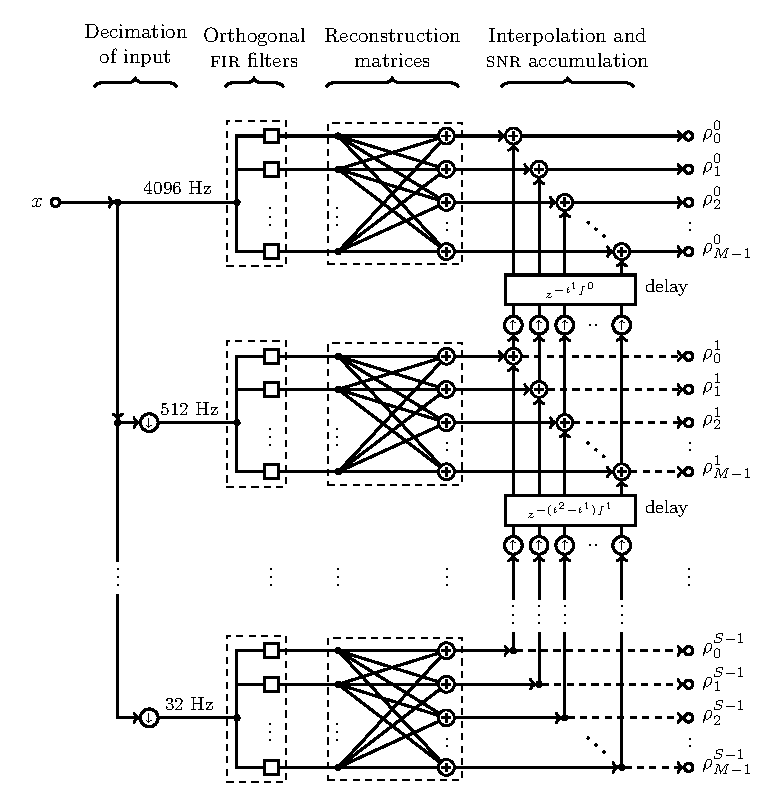
\includegraphics{figures/lloid-diagram}
		\caption{\label{fig:pipeline} Schematic of \lloid{} pipeline illustrating
signal flow.  Circles with arrows represent interpolation
\protect\includegraphics{figures/upsample-symbol} or decimation
\protect
\includegraphics{figures/downsample-symbol}.  Circles with plus
signs represent summing junctions
\protect\includegraphics{figures/adder-symbol}.  Squares
\protect\includegraphics{figures/fir-symbol} stand for \fir{} filters.  Sample
rate decreases from the top of the diagram to the bottom.  In this diagram each
time slice contains three \fir\ filters that are linearly combined to produce
four output channels.  In a typical pipeline the number of \fir\ filters is
much less than the number of output channels.}
	\end{center}
\end{figure*}
%
%
The signal flow diagram in Figure~\ref{fig:pipeline} illustrates this
recursion relation as a multirate filter network with a number of early-warning outputs.

In the next section we compute the expected computational cost scaling of this
decomposition and compare it with the brute-force \TD{} implementation of
\eqref{eq:SNRTD} and higher latency \FD{} methods.

\subsection{Comparison of computational costs}

We now examine the computational cost scaling of the conventional \TD{} or
\FD{} matched filter procedure as compared with \lloid{}.  For convenience,
Table~\ref{tab:recap} provides a review of the notation that we will need in
this section.
%
% symbols used in FLOPs calculations table
%
\begin{table}
\caption{\label{tab:recap}Notation used to describe filters.}
\begin{center}
\begin{tabular}{ll}
\tableline\tableline
& Definition \\
\tableline
$f^s$		& sample rate in time slice $s$ \\
\numtmps		& num. templates \\
\tmpsamps	& num. samples per template \\
\numslices	& num. time slices \\
\numsvdtmps	& num. basis templates in time slice $s$ \\
\slicessamps	& num. samples in decimated time slice $s$\\
$N^\shortdownarrow$ & num. coefficients in decimation filter \\
$N^\shortuparrow$ & num. coefficients in interpolation filter \\
\tableline
\end{tabular}
\end{center}
\end{table}


\subsubsection{Conventional \TD{} method}

The conventional \TD{} method consists of a bank of \fir{} filters, or sliding-window dot products.  If there are $\numtmps$ templates, each $\tmpsamps$ samples in length, then each filter requires $M N$ multiplications and additions per sample, or $2 \numtmps \tmpsamps f^0$ \flops\ at a sample rate $f^0$.

\subsubsection{Conventional \FD{} method}

The most common \FD{} method is known as the \emph{overlap-save} algorithm, described in
\citet{numerical-recipes-chapter-13}.  It entails splitting the input into blocks of $D$
samples, $D > \tmpsamps$, each block overlapping the previous one by $D - \tmpsamps$
samples.  For each block, the algorithm computes the forward \fft\ of the data and
each of the templates, multiplies them, and then computes the reverse \fft.

Modern implementations of the \fft, such as the ubiquitous \texttt{fftw}, require about
$2 \fftblock \lg \fftblock$ operations to evaluate a real transform of size
$\fftblock$~\citep{Johnson:2007p9654}.  Including the forward transform of the data and
$M$ reverse transforms for each of the templates, the \fft\ costs $2 (\numtmps + 1)
\fftblock \lg \fftblock$ operations per block.  The multiplication of the transforms adds
a further $2 \numtmps \fftblock$ operations per block.  Since each block produces
$\fftblock - \tmpsamps$ usable samples of output, the overlap-save method requires
$$
f^0 \cdot \frac{2 (\numtmps + 1) \lg \fftblock + 2 \numtmps}{1 - \tmpsamps/\fftblock} \; \mathrm{\flops} \,.
$$

In the limit of many templates, $M \gg 1$, we may neglect the cost of the forward
transform of the data and of the multiplication of the transforms.  The computational
cost will reach an optimum at some large but finite \fft\ block size
$\fftblock \gg \tmpsamps$.  In this limit, the \FD\ method costs
$\approx 2 f^0 \numtmps \lg \fftblock$ \flops.

\subsubsection{\lloid\ method}

For time slice $s$, the \lloid\ method requires $2 \slicessamps \numsvdtmps f^s$ \flops\ 
to evaluate the orthogonal filters, $2 \numtmps \numsvdtmps f^s$ \flops\ to apply the 
linear transformation from the $\numsvdtmps$ basis templates to the $\numtmps$ time-sliced templates, and $\numtmps f^s$ \flops\ to add the resultant partial \SNR\ stream.

The computational cost of the decimation of the detector data is a little bit more subtle.  Decimation is achieved by applying an \fir\ anti-aliasing filter and then downsampling, or deleting samples in order to reduce the sample rate from $f^{s-1}$ to $f^s$.  Naively, an anti-aliasing filter with $N^\shortdownarrow$ coefficients should demand $2 N^\shortdownarrow f^{s-1}$ \flops.  However, it is necessary to evaluate the anti-aliasing filter only for the fraction $f^s / f^{s-1}$ of the samples that will not be deleted.  Consequently, an efficient decimator that requires only $2 N^\shortdownarrow f^{s-1} \cdot \left( f^s / f^{s-1} \right) = 2 N^\shortdownarrow f^s$ \flops\ is possible.

The story is similar for the interpolation filters used to match the sample rates of the partial \SNR{} streams.  Interpolation of a data stream from a sample rate $f^s$ to $f^{s-1}$ consists of inserting zeros between the samples of the original stream, and then applying a low-pass filter with $N^\shortdownarrow$ coefficients.  The low-pass filter requires $2 M N^\shortdownarrow f^{s-1}$ \flops.  However, by taking advantage of the fact that by construction a fraction $f^{s-1}/f$ of the samples are zero, it is possible to build an efficient interpolator that requires only $M N^\shortuparrow f^{s-1} \cdot \left( f^s / f^{s-1} \right) = 2 M N^\shortuparrow f^s$ \flops.

Taking into account the decimation of the detector data, the orthogonal \fir\ filters, the reconstruction of the time-sliced templates, the interpolation of \SNR\ from previous time slices, and the accumulation of \SNR, in total the \lloid\ algorithm requires
\begin{multline*}
\sum_{\mathclap{s=0}}^{\mathclap{S-1}} \left( 2 \slicessamps \numsvdtmps + 2 \numtmps \numsvdtmps + \numtmps \right) f^s \\ + 2\sum_{\mathclap{f \in \{f^s\}}} \left( N^\shortdownarrow + \numtmps N^\shortuparrow \right) f^s
\end{multline*}
\flops.  The second sum is carried out over the set of distinct sample rates rather than over the time slices themselves.

We can simplify this expression quite a bit by taking some limits that arise from sensible filter design.  In the limit of many templates, the cost of the decimation filters is negligible as compared to the cost of the interpolation filters.  Typically, we will design the interpolation filters with $N^\shortuparrow \lesssim \numsvdtmps$ so that the interpolation cost itself is negligible compared with the reconstruction cost.  Finally, if the number of basis templates per time slices $\numsvdtmps$ is not too small, the reconstruction cost dominates over the cost of accumulating the partial \SNR.  In these limits, the cost of \lloid\ is dominated by the basis filters themselves and the reconstruction, totaling $2 \sum_{s=0}^{S-1} f^s \numsvdtmps \left( \slicessamps + \numtmps \right)$ \flops.

\subsubsection{Speedup of \lloid\ relative to \TD\ method}

If the cost of the basis filters dominates, and the frequency of the templates evolves slowly enough in time, then we can use the time-frequency relationship of equation~(\ref{eq:fgw}) to estimate the speedup relative to the conventional \TD\ method.  The reduction in \flops\ is approximately
%
\begin{multline}
\label{eq:speedup}
\frac{2 \sum_{s=0}^{S-1} f^s \numsvdtmps \slicessamps}{2 \numtmps \tmpsamps f^0} \\
\approx \frac{\alpha}{\left(t_\mathrm{low} - t_\mathrm{hi}\right) \left(f^0\right)^2} \int_{t_\mathrm{low}}^{t_\mathrm{hi}} \left(2 f(t) \right)^2 \, \mathrm{d} t \\
= \frac{16 \alpha \left(t_\mathrm{low} f^2 (t_\mathrm{low}) - t_\mathrm{hi} f^2 (t_\mathrm{hi}) \right)}{\left(f^0\right)^2 \left(t_\mathrm{low} - t_\mathrm{hi}\right)}
\end{multline}
%
where $\alpha \approx \numsvdtmps / \numtmps$ is the rank reduction factor, or ratio between the number of basis templates and the number of templates.  This approximation assumes that the frequency of the signal is evolving very slowly so that we can approximate the time slice sample rate as twice the instantaneous gravitational wave frequency, $f^s \approx 2 f(t)$, and the number of samples in the decimated time slice as the sample rate times an infinitesimally short time interval, $\slicessamps \approx 2 f(t) \, \mathrm{d}t$. The integral is evaluated using the power-law form of $f(t)$ from equation~(\ref{eq:fgw}). Substituting approximate values for a template bank designed for component masses around (1.4, 1.4) $M_\odot$, $\alpha \approx 10^{-2}$, $t_\mathrm{low} = 10^3$~s, $f_\mathrm{low} = 10^1$~Hz, $t_\mathrm{hi} = 1/1570$~s $f_\mathrm{hi} = 1570$~Hz, and $f^0 = (2)(1570)$~Hz, we find from equation~(\ref{eq:speedup}) that the \lloid\ method requires only $\sim 10^{-6}$ times as many \flops\ as the conventional \TD\ method.


\section{Implementation}

In this section we describe an implementation of the method described in
section \ref{label{sec:method}} suitable for rapid gravitational-wave searches
for compact binary coalescence.  The previous method requires several
computations that can be done before the analysis is actually underway.  Thus
we divide the procedure into two stages 1) an offline planning stage and 2) an
online, low latency filtering stage.  The offline stage can be done before the
analysis is started and updated asychronously, whereas the online stage must keep
up with the detector output and produce search results as rapidly as possible.
In the next two subsections we describe what these stages entail.

\subsection{Planning stage}

The choice of filter waveforms and singular value decomposition can be done in
advance and will be valid as long as the detector noise spectrum remains
roughly constant.  New filter waveforms can be computed asynchronously using
updated spectrum estimates as they are available. 

The planning stage begins with choosing templates that cover the space of mass
parameters with a hexagonal grid \cite{PhysRevD.76.102004} in order to satisfy
the minimum match criterion, which assures a user specified maximum loss in SNR
for signals that fall in-between the chosen templates.  Next, the templates are
subdivided into groups of neighbors called ``sub-banks'' that are appropriately
sized so that each bank can be efficiently handled by a single computer.
Dividing the mass space into smaller sub-banks also aids in the computational
cost of the singular value decomposition and is the approach considered
in~\cite{Cannon:2010p10398}.  Using our understanding of the time-frequency
evolution of the templates, we choose time slice boundaries as in \eqref{FIXME}
such that all of the templates within a sub-bank are sub-critically sampled at
progressively lower sample rates.  Next, the templates within the sub-bank are
realized as \textsc{fir} filter coefficients.  For each time slice, the
templates are downsampled to the appropriate sample rate.  Finally, the
\textsc{svd} is applied to each time slice in the sub-bank in order to produce
a set of orthogonal \textsc{fir} filters and a reconstruction matrix that maps
them back to the original templates as described in \eqref{FIXME}.  The
downsampled orthogonal \textsc{fir} filter coefficients, the reconstruction
matrix, and the time slice boundaries are all saved to disk.

\subsection{Filtering stage}

The filtering algorithm described in the previous section could be used in a
true sample-in-sample-out realtime system.  This would likely require a
nontrivial integration directly into the data acquisition and storage system of
the gravitational wave observatories.  A slightly more modest goal is to leverage
existing low latency, but not realtime, signal processing infrastructure in
order to implement the algorithm described in the previous section.   

We have implemented a prototype of the low latency filtering stage using an
open source signal processing environment called \gstreamer\ \cite{gstreamer}.
\gstreamer\ is a vital component of many Linux systems, providing media
playback, authoring, and streaming on devices from cell phones to desktop
computers to streaming media servers.  Given the similarities of gravitational
wave detector data to audio data it is not surprising that \gstreamer\ is
useful.  In our application, GStreamer excels at queueing, synchronizing,
adding, and bookkeeping many different signals at different sample rates.  It
also provides some useful signal processing elements such as decimators,
\textsc{fir} filters, and interpolators.  

\begin{figure}[htbp]
	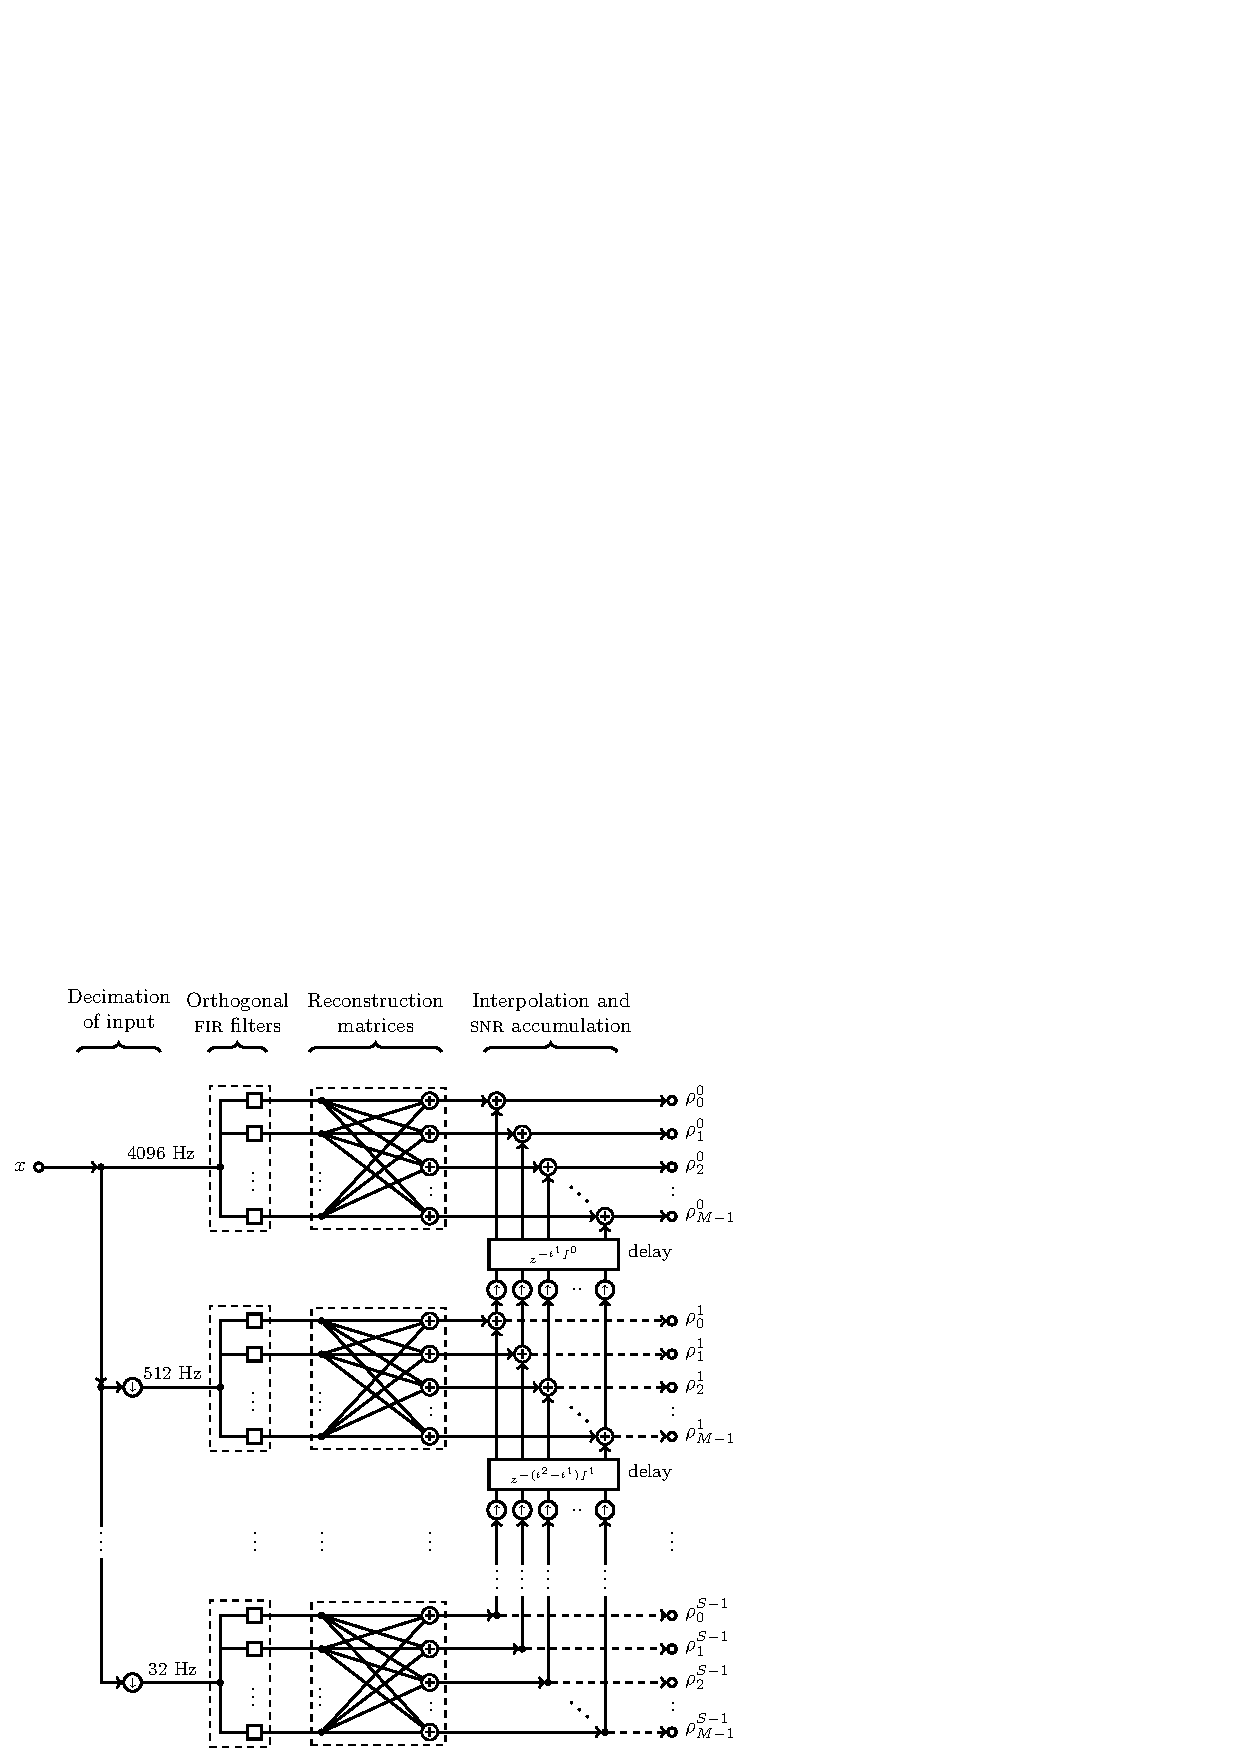
\includegraphics{figures/lloid-diagram.pdf}
	\caption{Schematic of LLOID pipeline illustrating signal flow.  Circles with arrows represent upsampling \protect\includegraphics{figures/upsample-symbol.pdf} or downsampling \protect
\includegraphics{figures/downsample-symbol.pdf}.  Circles with plus signs represent summing junctions \protect\includegraphics{figures/adder-symbol.pdf}.  Squares \protect\includegraphics{figures/fir-symbol.pdf} stand for FIR filters.  Sample rate decreases from the top of the diagram to the bottom.}
\end{figure}

The filter pipeline consists of six distinct stages.  

\subsubsection{Decimation}

First, the sample rate of the whitened detector data is reduced to successively
lower sample rates by decimation.  Decimation involves applying an antialiasing
filter to the data, and then downsampling by deleting samples.  We use a
192-tap \textsc{fir} decimator provided by {\tt Gstreamer's audioresample} element.
The detector data is provided at every power-of-two sample rate required by the 
template time sliced described in \ref{FIXME}. 

\subsubsection{Time delays}

Rather than implement the time sliced templates as zero padded \fir\ filters as
described in \eqref{FIXME} we instead implement them as shorter, but
appropriately time delayed \fir\ filters that contain only the nonzero samples.
In order to assure that we add the \SNR from the time slices adds appropriate


Each decimated detector data stream becomes the input for one time slice, but
it must be appropriately delayed.

\subsubsection{Orthogonal \textsc{fir} filters}

\subsubsection{Reconstruction}

\subsubsection{Interpolation}

\subsubsection{SNR accumulation}


\section{Results}
\label{SECIV}\label{sec:results}

In this section we test our implementation of the \lloid\ method using the
pipeline described in the previous section.  We answer the following questions
%
I) What is the measured loss of \SNR\ due to the approximations used in the
\lloid\ algorithm in a realistic analysis pipeline?
%
II) What is the measured latency of the implementation described in section
\ref{sec:implementation}?
%
III) What is the measured computational cost of the implementation described in
section \ref{sec:implementation}?

\subsection{Measured \SNR\ loss}

We expect two contributions to the \SNR\ loss to arise in our implementation of
the \lloid\ algorithm.  The first is the \SNR\ loss due to the truncation of
the SVD basis, which is fundamental, and estimates for it
exist~\cite{Cannon:2010p10398}.  The second comes from non ideal
implementations of resampling that cause signal loss.  We have measured the
effect of the resampling in the pipeline alone on a single waveform to gauge
the magnitude of the loss.  It is shown in figure \ref{fig:resamp_mm} as a
function of the quality of the {\tt audioresample} element (which is
proportional to the filter length used).  In both cases we have to compare the
\SNR\ loss to the expected \SNR\ loss that arises from the discreteness of the
template bank which is typically $\sim 3\%$.  We will consider a comparable
\SNR\ loss to be tolerable, but ideally would like to have a factor of 10 lower
loss from the \lloid\ implementation (i.e. no more than $\sim 0.3 \%$).  
%
\begin{figure}
\includegraphics{resamp_mm.pdf}
\caption{\label{fig:resamp_mm}Mis-match as a function of the {\tt
audioresample} element's filter length.  Increasing the filter length changes
the length of the sinc function filter that is used to decimate and interpolate
the data and filtered time series in our test pipeline.  Choosing a filter
length of 64 samples results in an acceptable loss of .2 \% in \SNR\ for the
chosen waveform.}
\end{figure}

\begin{figure}
	\label{fig:hist}
	\begin{center}
		\includegraphics{bw.pdf}
		\caption{Box-and-whisker plot of mismatch between nominal
template bank and \lloid\ measured impulse respones.  The \textsc{svd}
tolerance is varied from $\left(1-10^{-1}\right)$ to $\left(1-10^{-6}\right)$.
The whiskers denote the minimum and maximum mismatch over all templates.  The
diminishing improvement is caused by hitting the resampling match limit.}
	\end{center}
\end{figure}


\subsection{Measured latency}

In order to check the latency of our implementation of the \lloid\ algorithm we
used the pipeline described in \ref{fig:pipeline} with a live source connected
to the input.  We then measured the timestamp of the live source and the output
of the final \SNR\ time series.  Since \gstreamer\ is not a
sample-in-sample-out realtime infrastructure, it does work by passing small
buffers of data and filtered data through the pipeline.  We set the buffer size
on the input to be 1/4 s.  In an ideal case the latency should be nearly 1/4 s.
However, it is necessary to queue things in the pipeline to assure that there
are no issues with threading. Sometimes buffers get delayed.  We measured the
average filtering latency to be \FIXME{1 s}.

\subsection{Measured computational cost}

Using the pipeline described previously, we also measured the computational
cost.  We used an 8 socket, quad core AMD\texttrademark\ machine operating at
2.7 GHz per core.  We found that filtering \FIXME{657} templates in real time
required about \FIXME{6} of the available cores.  We thus conclude that we
require about 1 core for every \FIXME{100} templates.  We note that this is
well within the computational limits of a modern, computing cluster assuming
that the scaling holds for the entire mass range of interest, we would need
about \FIXME{300} cores per detector.  This requirment should be even less of a
burden in the advanced detecor era, when presumably clusters built in that era
will have a factor of 4 or 8 more cores than the ones today. 



\section{Conclusions}
\label{SECV}\label{sec:conclusions}

\editorial{We should drive home the point that our method is as fast as the fft convolution but without any latency at all.}%
We have demonstrated a computationally feasible procedure for the rapid and even advance
detection of gravitational waves emitted during the coalescence of neutron
stars and stellar-mass black holes.  These sources are expected to produce
prompt electromagnetic signals and may be the progenitors of some short hard
gamma-ray bursts.  Rapid alerts to the broader astronomical community may
improve the chances of detecting an electromagnetic counterpart in bands from
X-ray down to radio.  We anticipate requiring $\sim$\numcpus\ modern
%
\editorial{We need to do this calculation using the \flops\ counts and the
number of templates. CHAD: Agreed, but if you do it by the books it seems
misleading.  I have adjusted it to 600.  This number is taken from assuming
that 1 657 template sub-bank can be filtered on one core and dividing the total
number of templates (10$^5$) by 657 which gives you 150 cores per detector. I
put it in section 2. }%
%
computer cores to analyze a four-detector network of gravitational-wave data
for binary neutron stars and stellar mass black holes.  This is within the
current computing capabilities of the \textsc{lsc} Data Grid~\cite{LDG}.

The algorithm we described has no intrinsic latency.  However, there are
fundamental and practical latencies associated with the analysis and detection
procedure. For example, the \LIGO{} detectors, data acquisition is synchronized
to a 1/(16~Hz) cadence introducing an up-front latency.  Data
aggregation from the observatories will travel over various networks, each
capable of high bandwith but perhaps only modest latency.  This could amount to
a similar latency of $\sim$100 ms.  Lastly, unless a realtime infrastructure is
adopted post data acquisition, it is likely that there will be an inherent
latency introduced by such infrastructure.  We have shown a prototype
implementation using \gstlal\ that is capable of $\sim$1 s latency. In our
opinion, significant work would have to be done in order to improve upon this
number. However, it should be considered for third-generation detector design.
For example, a tighter integration of analysis and data acquisition would be
beneficial.

\editorial{The way this is worded, it sounds like a big omission.}%
We have omitted discussion of source localization though point
the reader to some theoretical estimates \SNR~\cite{Fairhurst2009}.
%However, one should not immediately dismiss the practical usefulness of a
%poorly localized source. Even with poor localization, it should be possible to
%begin downselecting what observatories could view a potential signal and for
%such observatories to begin any necessary prerequisite activities. 
In future works we will explore more rigorously the pointing prospects with
realistic simulations using the infrastructure and techniques described here.
\editorial{nvf: It's a bit pie-in-the-sky, but we could also mention reconfiguring
the signal recycling mirror to optimize SNR at merger. There's a lot of science there.}

%Latency budget, including `before' and `after' quotes for:

%\begin{itemize}
%\item Data acquisition
%\item Calibration
%\item Data aggregation
%\item Analysis
%\item Localization
%\item Alert
%\item Telescope actuation
%\item Total
%\end{itemize}

%Future work:

%\begin{itemize}
%\item Sub-solar mass search
%\item Hierarchical detection
%\end{itemize}


\ack{\textsc{ligo} was constructed by the California Institute of Technology and Massachusetts Institute of Technology with funding from the National Science Foundation and operates under cooperative agreement \textsc{phy}-\oldstylenums{0107417}. This paper has \textsc{ligo} Document Number \textsc{ligo}-\textsc{p}\oldstylenums{0900004}-v\oldstylenums{1}.

\appendix
\section{Filter bank for generating mock Advanced {\sc ligo} strain data}
\label{appendix:mock-data}

The filter bank described below reproduces the ``zero detuning, high power'' Advanced \textsc{ligo} noise model of  \cite{Shoemaker:2009p9770} very faithfully.  Since it is composed of a small number of third order or lower linear filters, a digital implementation of it can produce mock data in realtime with negligibly few floating point operations.

First, generate 5 independent streams of white Gaussian noise, $x_1, \dots, x_5$, sampled at 16384 Hz.  Next, the apply the (\textsc{f}/\textsc{i})\textsc{ir} filters described in equation~(\ref{eq:iirbank}) to generate $y_1, \dots, y_5$ from $x_1, \dots, x_5$ respectively.  Finally, sum and scale all of the $y_1, \dots, y_5$ together to obtain the final output $y$.

The power spectrum of $y$ is the sum of squares of the magnitudes of the transfer functions of all of the filters.  The output of the filter bank is compared with the noise model in Figure~\ref{fig:mock-psd} below.

The mock Advanced \textsc{ligo} noise generator is implemented by the GStreamer element \texttt{lal\_fakeadvligosrc}, which is included with the analysis code.

\begin{eqnarray}
\label{eq:iirbank}
\fl x_i &[n] \sim& \mathcal{N}[0, 1] \quad \forall \, i, n \nonumber\\\noalign{\vskip 2mm}
\fl y_1 &[n] =& \left(4 \times 10^{-28}\right) x_1[n] - y_1[n-1] + 2 \cdot 0.99995 \cos \left(\frac{2\pi \cdot 9.103}{16384}\right) y_1[n-2] - 0.99995^2 y_1[n-3] \nonumber\\\noalign{\vskip 2mm}
\fl y_2 &[n] =& \left(1.1 \times 10^{-23}\right) (x_2[n] - x_2[n-1]) \nonumber\\\noalign{\vskip 2mm}
\fl y_3 &[n] =& \left(10^{-27}\right) x_3[n] - y_3[n-1] + 2 \cdot 0.999 y_3[n-2] - 0.999^2 y_3[n-3] \nonumber\\\noalign{\vskip 2mm}
\fl y_4 &[n] =& \left(4 \times 10^{-26}\right) x_4[n] - y_4[n-1] + 2 \cdot 0.87 \cos \left(\frac{2\pi \cdot 50}{16384}\right) y_4[n-2] - 0.87 ^ 2 y_4[n-3] \nonumber\\\noalign{\vskip 2mm}
\fl y_5 &[n] =& \left(6.5 \times 10^{-24}\right) x_5[n] - y_5[n-1] - 2 \cdot 0.45 y_5[n-2] - 0.45 ^ 2 y_5[n-3] \nonumber\\\noalign{\vskip 2mm}
\fl \; y &[n] =& \frac{3\sqrt{16384}}{4} \left(y_1[n] + y_2[n] + y_3[n] + y_4[n] + y_5[n]\right)
\end{eqnarray}

\begin{figure}[h!]
\begin{center}
\includegraphics[scale=0.4]{mock_psd.pdf}
\caption{Power spectrum of 100 s of output from mock data filter bank compared with the ``zero detuning, high power'' Advanced \textsc{ligo} noise model.}
\label{fig:mock-psd}
\end{center}
\end{figure}

Note that the \textsc{cpu} overhead of this procedure will be entirely dominated by drawing the pseudorandom numbers $x_1, \dots, x_5$.


\section{Floating point operation counts}

Each addition and each multiplication is counted as a single floating point operation.   We are not assuming that a multiply-accumulate is available as a single operation.

\begin{table}[htdp]
\caption{Number of floating point operations per sample (multiplications and divisions) required for a selection of signal processing operations used in \textsc{lloid}.}
\begin{center}
\setlength{\extrarowheight}{6pt}
\begin{tabular}{l c}
\hline
Process & ops/sample \\
\hline\hline
\textsc{fir} matched filter, M templates of length $n$ & $2 M n$ \\\hline
\textsc{fft} matched filter, M templates of length $n$, blocks of length $D$ & $\frac{4 (M + 1) \lg D + 2 M}{1 - n/D}$ \\\hline
$n$ tap \textsc{fir} resampling filter, sample rates $f_1 < f_2$ & $2 M n f_1 / f_2$ \\\hline
multiply $M \times L$ real matrix by $L\times1$ real vector & $2 M L$ \\\hline
\end{tabular}
\end{center}
\label{table:flops}
\end{table}%


The filter bank can be implemented using finite impulse response (\textsc{fir}) filters, which are just sliding window dot products.  If there are $M$ templates of length $n$, and the data stream contains $N$ samples, then applying the filter bank requires $2 M N n$ operations.

More commonly, the matched filters are implemented using the \textsc{fft} convolution.  This entails applying \textsc{fft}s to blocks of $D$ samples, with $2 n \leq D$, each block overlapping the previous one by $n$ samples.  There are $N/(D-n)$ such blocks.  Modern implementations of the Cooley-Tukey \textsc{fft}, such as the ubiquitous \texttt{fftw}, require about $4 N \lg N$ operations to evaluate a \textsc{dft} of size $N$~\cite{Johnson:2007p9654}.  \editorial{This is more commonly known as ``overlap-save''.  We should find someone else's operation count and cite it.}  A $D$ sample cross-correlation consists of a forward \textsc{fft}, an $D$ sample dot product, and an inverse \textsc{fft}, totaling $8 D \lg N + 2 D$ operations per block.  Per sample, this is $(8 \lg D + 2) / (1 - n/D)$ operations. \editorial{Drew: Why don't we change this to an overlap of $m$ samples so we can see what happens as we increase the overlap to reduce latency.}

The \textsc{fir} filter implementation has the advantage that it has no intrinsic latency, whereas the \textsc{fft} convolution has at least the latency of the \textsc{fft} block size $D \geq 2 n$.  \editorial{Drew: Should the latency be D-n?} For example, for a $1.4 - 1.4 \, M_\odot$ template with duration $\sim 1 \, \mathrm{ks}$, the \textsc{fft} convolution has a latency $\geq 2 \, \mathrm{ks}$.  However, the \textsc{fir} filter implementation has the disadvantage of much greater overhead per sample than the \textsc{fft} convolution.  For a $1\,\mathrm{ks}$ template sampled at $4096\,\mathrm{Hz}$, the \textsc{fir} implementation requires about about $n / 8 \lg 2 n = 2.2 \times 10^4$ times more operations per sample than the \textsc{fft} implementation.



\begin{comment}
% Let's make glitch rejection in LLOID a separate paper.

\section{better noise model}

The assumption that the interferometer noise is well-modeled by a multivariate normal distribution is convenient, but false.  The presence of `glitches' in the interferometer, where the noise statistics change dramatically, is well documented.  Current methods, including ours in the form proposed in the paper, are easily fooled by these bursts of excess power, simply because the analyses assume that the only way that extra power can be introduced to the interferometer is by a gravitational wave.  The gravitational wave hypothesis $H_\mathrm{signal}$ will do a very poor job of explaining temporally coincident incoherent bursts of noise power in the interferometer, but the noise hypothesis $H_\mathrm{signal}$ in its simple form does even worse; the gravitational wave explanation is thus preferred.

We can generalize the noise hypothesis to cope with glitches by creating a model for glitches and adding that hypothesis to the set under consideration.  Like gravitational waves, glitches are infrequent, have poorly known waveforms, and poorly known power.  Unlike gravitational waves, they will not be correlated between instruments.

%The Gursel-Tinto method is not robust against interferometer glitches (nor does it claim to be; real interferometer data doesn't follow the normal distribution assumed in the derivation of the method.)  This is a problem in naive attempts to use the Gursel-Tinto algorithm as a search.  Excess energy of any almost any kind will be interpreted as a evidence of a gravitational wave.  An \emph{ad hoc} addition to the method was propsed in \cite{us}.  A better way forward is to use a noise model that more accurately reflects the 'bursty' or 'glitchy' nature of the data, by replacing the normal noise distribution with a long-tailed distribution.  An immediate problem is that the marginalization integral does not in general have a closed form solution for such distributions.  If we model the long-tailed distribution using two normal distributions the marginalization integral remains tractable.

One first attempt at such a hypothesis is to propose that an interferometer is either `quiet' with some probability $p(H_\mathrm{quiet}|H_\mathrm{noise})$ and has a unit normal noise distribution, or is `glitching' with probability $p(H_\mathrm{glitch}|H_\mathrm{noise})$ and has an increased standard deviation $\sigma_g$

\begin{equation}
P(\mathbf{x}|H_\mathrm{noise})
=
\prod_{i=1}^{N}\left[p(H_\mathrm{quiet}|H_\mathrm{noise})
(2\pi)^{-n/2}
\exp(-\frac{1}{2}\sum_{j=1}^n x_{ij}^2)
+p(H_\mathrm{glitch}|H_\mathrm{noise})
(2\pi)^{-n/2}\sigma_g^{-n}
\exp(-\frac{1}{2\sigma_g^2}\sum_{j=1}^n x_{ij}^2)
\right]\label{eq:glitchy}
\end{equation}

If there is excess energy in only one detector, the new noise hypothesis will readily explain it.  If there is excess energy in three detectors, the noise hypothesis must invoke three coincident glitches and is penalized by $p(H_\mathrm{glitch}|H_\mathrm{noise})^3$ reflecting our belief that triple-coincidence glitches are rare, and the prediction that the glitches are incoherent thinly spreads the hypothesis over a higher-dimensional space than that of the signal hypothesis, which is concentrated around $\mathrm{span}\,\mathbf{F}$. These factors make it possible for the gravitational wave hypothesis to be preferred for some data.

\end{comment}

%Instrumental glitches (hereafter, just `glitches') correspond to noise components with a greater variance than the stationary instrumental noise.

%\label{marg} The evidence for model 1 is most easily calculated in
%the original basis, where the detectors are separable.  In this
%model we assume the glitch or noise outputs of the detectors are
%uncorrelated, so that the overall evidence is simply the product of
%the evidences from each:
%
% \begin{align}
% p(d_i|M_1) &= \int p_i(\sns|M_1)p(d_i|\sns,M_1)\,{\rm d}\sns\\
%            &= \frac{1}{(2\pi)^{1/2}}\left[(1-\alpha_i)\exp(-d_i^2/2) + \frac{\alpha_i}{g_i}\exp(-d_i^2/2g^2)
%            \right],
% \end{align}
%so that
% \begin{align}
% p(\vec{d}|M_1) &= \prod_i p(d_i|M_1)\\
%                &= \frac{1}{(2\pi)^{3/2}}\prod_i \left[(1-\alpha_i)\exp(-d_i^2/2) + \frac{\alpha_i}{g_i}\exp(-d_i^2/2g^2)
%                \right].
% \end{align}

%\begin{widetext}

%Similarly the evidence for model 2 comes straight from
%Eqn.~(\ref{lik2}) by setting $\shs$ to $s^2$,  and $\sns$ to unity,
%so that the overall Bayes factor for a signal to be present is
% \be
% B_{21}=\frac{\exp\left\{ - (\vfph.\,\vec{d})^2/[2(1+s^2|\vfp|^2)]
%                          - (\vfch.\,\vec{d})^2/[2(1+s^2|\vfc|^2)]
%                          - (\vkh\,.\,\vec{d})^2/2 \right\}}
%{[(1+s^2|\vfp|^2)(1+s^2|\vfc|^2)]^{1/2} \prod_i
%\left[(1-\alpha_i)\exp(-d_i^2/2) +
%\frac{\alpha_i}{g_i}\exp(-d_i^2/2g^2)\right]}.
% \label{bayes}
% \ee
%Using the orthogonality relation
% \be
% |\vec{d}|^2 = (\vfph.\,\vec{d})^2 + (\vfch.\,\vec{d})^2 +
% (\vkh\,.\,\vec{d})^2,
% \ee
%this same result may be written in terms of power components in the
%$(\fp,\fc)$-plane and in the total power $ |\vec{d}|^2$:
% \be
% B_{21}=\frac{\displaystyle\exp\left\{ \frac{1}{2}\frac{s^2|\vfp|^2}{(1+s^2|\vfp|^2)}(\vfph.\,\vec{d})^2
%                         +\frac{1}{2}\frac{s^2|\vfc|^2}{(1+s^2|\vfc|^2)}(\vfch.\,\vec{d})^2
%                          \right\}}
%{[(1+s^2|\vfp|^2)(1+s^2|\vfc|^2)]^{1/2} \displaystyle\prod_i
%\left\{(1-\alpha_i)\displaystyle\exp\left(-\frac{d_i^2}{2}\right) +
%\displaystyle\frac{\alpha_i}{g_i}\displaystyle\exp\left[\frac{1}{2}\left(1-\frac{1}{g_i^2}\right)d_i^2\right]\right\}}.
% \ee
%
% Consider the simplified scenario in which model 1 assumes all three
%detectors are currently glitching, so that $\alpha=1$, and where the
%characteristic glitch power is the same in each, so that
%$g_i^2=g^2$. The Bayes factor is now comparing the idea that (1) we
%are seeing a triple-coincidence glitch with (2) we are seeing a
%gravitational wave, and Eqn.~(\ref{bayes}) reduces to
% \be
% B_{21}=\frac{g^3\exp\left\{\displaystyle \frac{|\vec{d}|^2}{2g^2} -
% \left[\frac{(\vfph.\,\vec{d})^2}{2(1+s^2|\vfp|^2)}
%                          +
%                          \frac{(\vfch.\,\vec{d})^2}{2(1+s^2|\vfc|^2)}
%                          + \frac{(\vkh\,.\,\vec{d})^2}{2}\right] \right\}}
%{[(1+s^2|\vfp|^2)(1+s^2|\vfc|^2)]^{1/2} }.
% \ee
%The exponent is simply the difference between the chisquared
%statistic for a glitch of mean power $g^2$ and that for a
%gravitational wave signal of mean power $s^2$.  The other terms
%represent an Occam factor, reflecting the difference in the sizes of
%the competing hypothesis spaces.
%
%The same expression can be written as
% \be
% B_{21}=\frac{g^3\exp\left[ %\displaystyle
%              \frac{1}{2}\left(\frac{1}{g^2}-\frac{1}{1+s^2|\vfp|^2}\right)(\vfph.\,\vec{d})^2
%             +\frac{1}{2}\left(\frac{1}{g^2}-\frac{1}{1+s^2|\vfc|^2}\right)(\vfch.\,\vec{d})^2
%             -\frac{1}{2}\left(1-\frac{1}{g^2}\right) (\vkh\,.\,\vec{d})^2 \right]}
%         {[(1+s^2|\vfp|^2)(1+s^2|\vfc|^2)]^{1/2} },
% \ee
%to highlight the fact that power in the null-stream direction $\vkh$
%always reduces $B$.

%\end{widetext}


\section*{References}

\bibliographystyle{unsrt}
\bibliography{references}

\end{document}
